\documentclass[letterpaper,10pt, jcp, aps]{revtex4-1}

\usepackage[utf8]{inputenc}
\usepackage{amsmath, amsfonts}
\usepackage{graphicx}
\usepackage{natbib}
\usepackage{caption}
\usepackage{subcaption}
%\usepackage{authblk} parece ser que ya esta metido cuando usas preprint




%\bibliographystyle{alpha}

%opening

%\author{Rosa Rodríguez \& David P.~Sanders \& W. P. K. Zapfe}
%\affil{Departamento de Física, Facultad de Ciencias, Universidad Nacional Autónoma de México, Ciudad Universitaria, Del.~Coyoacán, México D.F. 04510, Mexico}

\usepackage{mathptmx}
% I dont know if that package is compatible with revtex.

\newcommand{\defeq}{:=}
\newcommand{\mean}[1]{\left \langle #1 \right \rangle}
\newcommand{\rd}{\!\mathrm{d}}
\newcommand{\RR}{\mathbb{R}}
\newcommand{\vv}{\mathbf{v}}
\newcommand{\indicator}[1]{\mathbf{1}_{ \{   #1 \} } } 
\newcommand{\etal}{\emph{et al.\ }} 

\setlength{\parskip}{10pt}
\setlength{\parindent}{0pt}


\begin{document}

\title{Exact Mean Event Times for the Two Disks in a Box Billiard Model}

\author{Rosa Rodríguez}
\email{sepaeldiablo@notengoidea.org}
\affiliation{ Also Facultad de Ciencias? Current affiliation?}

\author{David P. Sanders}
\email{sanders@ciencias.unam.mx}
\affiliation{Facultad de Ciencias, UNAM.}

\author{W. P. Karel Zapfe}
\email{karelz@fis.unam.mx}
\affiliation{CINVESTAV IPN}


\begin{abstract}
Using Ergodic Theory formulae, we have obtained 
exact expressions for various  mean event times in the Two Disks in a Box
billiard.  We have shown that the general formula is applicable in a very broad range
of situations and the only difficulty is establishing the adequate surface
of section and its measure, so that it represents  the event in question. 
We have compared this results against
numerical simulations and we have compared them also against first event times.
The second case has no closed expression that we are aware of, but shows
very similar behavior, although it has clear deviations.   
\end{abstract}

\maketitle



\section{Introduction}

\typeout{`` this is ``  \the\columnwidth }

For the statistical physicist and theoretical
chemist, \emph{mean} and \emph{first} event
times are of uttermost importance, as many properties,
such as mixing, reaction and diffusion rates depend on it. 
Two events can model the fundamental occurrences of
these kind of problems. One is the \emph{hopping},
in which two particles interchange position along some
axis of interest, and the other
is the \emph{collision} of said particles. 
A highly simplified model which has been successfully  used for
this research consist in two disks inside a rectangular
box \cite{Awazu01, Munakata02, Suh05}.

Previous work
by Bowles \etal shows general quantitative results for the hopping 
mean time for inertial and Brownian dynamics \cite{Bowles04}. 
They use arguments derived from Transition State Theory 
to provide expressions for the
general behaviour of these quantities, as functions of the
radius of the disks. Their results show the adequate algebraic behaviour.
A great deal of work has expanded along that line  \cite{Suh05, Ball09}.
There is also a statistical thermodynamic treatment by Munakata \etal 
which deals very comprehensively with partition functions, pressure,
and temperatures \cite{Munakata02, Munakata06}. 
Our  primary intention is
to find  the mean hopping and collision times of the two disks under 
inertial motion and compare them with first hopping and collision times.
We show that the former can 
be obtained  as a closed analytic expression dependant only
on the geometric parameters of the system, which turns 
out to be a rational function whose limiting form
has the algebraic exponent predicted in the aforementioned literature, while
the later follows closely the first, but with appreciable
qualitative differences. 

The exact treatment  turns to be  feasible because  
the reduced model is a hard sphere billiard. 
Such systems  are one of the most recurred models for
statistical physics and  traditionally, for non linear dynamics.  
Some of these simple models
 provide us with a deep mathematical understanding
about  the properties collectively called  \emph{Hard Chaos} 
(hyperbolicity, ergodicity and mixing qualities \cite{Sinai70, Gallavotti74}). 
One such system is the
gas of disks in a rectangular box \cite{SzaszBook00}, 
for which the simplest non trivial
realization is the case of  two disks inside the box, our
present model.
This billiard is chaotic in
strong sense \cite{Sim99}. The system  is thus amenable
to analytic treatment
and rigorous results have been obtained from ergodic theory \cite{MarkChern}.

The previous  results on
inertial dynamics can be extended  by particularizing 
exact expressions for the mean return times (MRT). 
We shall  obtain them through application of 
Machta and Zwanzig formula for residence times \cite{MachtaZwan}. 
We shall also  compare \emph{mean event times} with 
\emph{mean first event times} (MFET),
and give some arguments to explain the agreement between the two. 
Brownian dynamics shall be discussed elsewhere \cite{WorkInProgress}.
%We shall also provide this paper with supplementary material 
%detailing the calculations. 



\section{Model}


% Voy a quitar todas las referenacias a la variable $d$ y el díametro
% nadamas nos están estorbando en las formulas y fastidiar al lector
% con una caracterización redundante del disco es mala onda.
We consider two discs of radius $r$  %(and diameter $d=2r$) 
in a box of width $w$ and height $h$ (figure\ref{billar01}). 
The discs move inertially in the absence of forces, 
following straight line trajectories,
and undergo elastic collisions with each 
other and with the walls of the box.
We take the mass of each disk as unitary; the kinetik energy
is the value of the Hamiltonian function inside the billiard table:
\begin{equation}
H(q,p)=\frac{1}{2}(\|p_1\|^2+\|p_2\|^2)=1.
\end{equation}

\begin{figure}[h]
  \begin{center}
  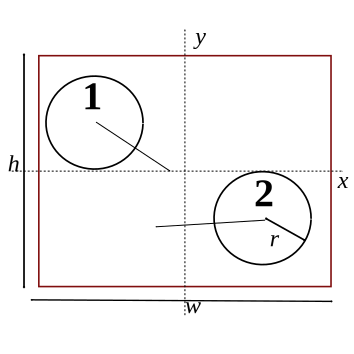
\includegraphics[width=0.40\textwidth]{DiscosenCajaCuadrada01.pdf}
  \end{center}
  \caption{The billiard and its parameters. Coordinates
    have their origin at the geometrical centre of the 
    billiard table.}\label{billar01}
\end{figure}

We denote the position of the centre of the $i$th disc by 
$(x_{i}, y_{i})$ for $i=1,2$. Since the discs are hard, 
the disc centres are restricted to the region 
$(x_i, y_i) \in [-a,a] \times [-b, b]$, where 
$a \defeq a(r) \defeq \frac{w}{2} - r $ and
$b \defeq b(r) \defeq \frac{h}{2} - r $.


The exclusion condition is $(x_1-x_2)^2 + (y_1-y_2)^2 \ge (2r)^2 = d^2$.
It is thus useful to work in terms of the new coordinates
\begin{equation}\label{cambiocoor01}
 x \defeq \frac{x_1 - x_2}{\sqrt{2}}; 
\quad X \defeq \frac{x_1 + x_2}{\sqrt{2}}; 
\quad y \defeq \frac{y_1 - y_2}{\sqrt{2}}; 
\quad Y \defeq \frac{y_1 + y_2}{\sqrt{2}}.
\end{equation}

%%This is WRONG, or better, is not precise enough.
In these coordinates the configuration space is given by the following
intervals:
$x \in [-a \sqrt{2}, +a \sqrt{2}]$ with 
$X \in [-a \sqrt{2} + |x|, a \sqrt{2} - |x|]$, respectively 
 $y \in [-b \sqrt{2}, b \sqrt{2}]$ with $Y \in [-b \sqrt{2} + |y|, +b \sqrt{2} - |y|]$,  
and the constraint $x^2 + y^2 \ge 2 r^2$ that precludes the overlaping of
the discs.
The horizontal and vertical coordinates transform independently
from each other, and the Jacobian is in each case equal to $1$.

The constrains define a four dimensional
rectangular prism, called the prism henceforth,   
and a four dimensional cylinder placed inside.
This cylinder has radius $r\sqrt{2}$ and lies
in  a diagonal position along the axes $X, Y$.
The prism surface is the outer boundary of the configuration space,
while the cylinder is the excluded volume, and its surface
acts as a reflecting inner boundary.
The dynamics in this space follow
the usual billiard rules: free flight until
encounter with a wall, then elastic reflection.
The outer borders are flat, so the
hyperbolicity is due to the inner dispersing
boundary \cite{Sim99}, which represents the collision of
two disks in the original space.


\section{Mean time between events}


\subsection{Known Facts of the Collision Rates}

A system of $N$ hard spheres confined by hard walls in a $D$ dimensional
space may be treated as a billiard system 
in which a single point  particle undergoes free motion between reflecting obstacles 
in a $ D N $-dimensional configuration space \cite{Sinai70, Sim99, MarkChern}. 
If the resulting billiard is ergodic and hyperbolic, then we know that
these systems are equivalent to Bernoulli Flows \cite{Gallavotti74}.
For such systems is expected an exponential decay of 
distributions \cite{AbadiGalves} with potentially
long algebraic tails \cite{ZasTip}. 
This includes recurrence times and
first encounter times. We also
have a result for the mean free time, i.e.\ the mean time between 
collisions of the particle with the walls \cite{MarkChern}. 
This can be thought of as a mean return time to the $(D-1)$-dimensional 
(i.e. co-dimension $1$) cross-section given by the wall boundaries.
The general formula for that time is
\begin{equation}\label{meanfreetime}
 \mean{\tau} = \frac{|Q|}{|A|} \frac{|S^{D-1}|}{|B^{D-1}|}.
\end{equation}
Here $|Q|$ denotes the $D$-dimensional volume of the available 
space in the billiard and 
$|A|$ the $(D-1)$-dimensional area of the cross-section.
 $|S^{D-1}|$ is the $(D-1)$-dimensional area of the unit sphere in $\RR^D$ given by
\begin{equation}
  |S^{D-1}| = \frac{2 \pi^{D/2}}{\Gamma(D/2)},
\end{equation}
where $\Gamma(\cdot)$ is the gamma function. 
$|B^{D-1}|$ is the volume of the unit ball 
in $\RR^{D-1}$, given by $|B^{D-1}| = |S^{D-2}| / (D-1)$.
In the formula \ref{meanfreetime}  the particle has 
its velocity scaled to unity.

Machta and Zwanzig \cite{MachtaZwan} used a similar method to derive an escape 
time across a non-existent boundary by treating it as a recurrence time.
%Since it is an escape time, they used velocities whose components point only 
%perpendicularly to the ``exit wall''.
In our case, we are mainly interested in the mean return time to 
a co-dimension-$1$ cross section, 
which is defined by the exact moment
in which the disk interchange their horizontal position. This is simply
\begin{equation} \label{condchoque}
x_1 = x_2.
\end{equation}
We call such an event a ``hopp''. Other first events shall also be studied
to test the robustness of the methods followed here.

Given that each disk has different momentum, but
they can interchange it without affecting the
total energy, we take into account the mass $m$ of each disk 
and the total kinetic energy $E$.
If both discs have the same mass then $\sum_i \vv_i^2 = 2E / m$.
The above result, as derived by Chernov, 
was for the case $\sum_i \vv_i^2 = 1$, or $m=1$ and $E=\frac{1}{2}$.  
For more general values of $E$ and $m$, 
we are simply working on a different energy surface in phase space. 
The particle trajectories are identical but the motion is different
by a factor of
$\sqrt{2E/m}$. All times must divided by this value, 
giving for
the mean time between events the general formula:
\begin{equation} \label{meantimegeneral}
  \mean{\tau} =  \frac{1}{\sqrt{2E / m}} 
\frac{|Q| \, |S^3|} {|A| \, |B^3|}.	
\end{equation}
In our particular case, the effective dimension is four,
and $E=m=1$, so that the general factor of the formula appear as:
\begin{equation} \label{meantimegeneralredux}
   \frac{1}{\sqrt{2E / m}} 
\frac{|S^3|}{|B^3|}=\frac{3\pi}{2\sqrt{2}}.	 
\end{equation}

The next step is obtaining the Volume (4 dimensional measure) of
the available space and the Area (3 dimensional induced measure) of
the collision conditions. We devote the next section to
detail the procedure.


\section{Calculation of Volumes and Areas}

The configuration
space is an four dimensional prism with a four dimensional
cylinder subtracted.
The calculation can be carried out indirectly,
 using indicator functions for the
available space or for the prohibited space.

\subsection{Volume of available space}

We shall present the total four-dimensional volume as a product integral
of all available positions. To grasp the idea, a 
diagram is shown in Figure \ref{diagintegra01}. Our
principal integral is the available free $4D$ volume, which 
we shall denote $V_\text{free}$:
\begin{multline}\label{volindic}
 V_\text{free} = \\ \int\limits_{x_1 = -a}^a \rd x_1 \int\limits_{x_2 = -a}^a \rd x_2 
\int\limits_{y_1 = -b}^b \rd y_1 \int\limits_{y_2 = -b}^b \rd y_2 \, \indicator{ (x_1-x_2)^2 + (y_1-y_2)^2 \ge (2r)^2 },
\end{multline}
where $\indicator{Z}$ indicates the indicator function of the set $Z$, 
given by $\mathbf{1}_Z (x) = 1$ if $x \in Z$, and $=0$ if $x \notin Z$, 
which restricts the integral to the desired region $Z$.
\begin{figure}[h]
  \begin{center}
    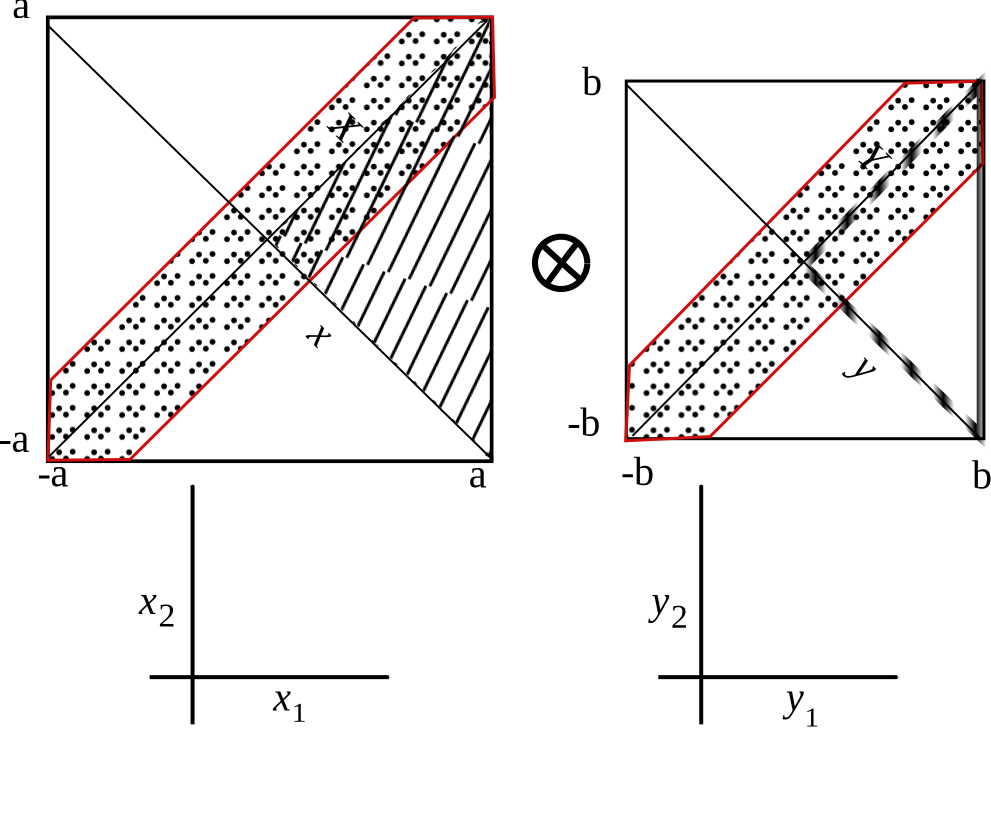
\includegraphics[width=0.45\textwidth]{diagramintegra01.pdf}
  \end{center}
  \caption{The space to integrate is the product of the subspaces
    belonging to horizontal and vertical coordinates. The colour
    bands represents the ``exclusion'' set, where the condition 
    $ (x_1-x_2)^2 + (y_1-y_2)^2 \ge d^2 $ is not met. 
    The width of each band is dependent on the particular 
    point of evaluation
    on the \emph{other} subspace. The diagonal coordinates
    make the expression to evaluate simpler. Due to 
    symmetry, we only evaluate the area in stripes and
    multiply the result by 16.}\label{diagintegra01}  
\end{figure}

It is easier to represent the  
excluded cylinder in the coordinates defined in 
the set of equation \ref{cambiocoor01}. Then the exclusion condition
is orthogonal to the coordinates $X,Y$ and they do not appear
on the indicator function. 
\begin{multline}\label{integraltotal}
 V_\text{free} = \\ \int\limits_{x=-a \sqrt{2}}^{a \sqrt{2}} \rd x 
\int\limits_{X=-a \sqrt{2} + |x| }^{a \sqrt{2} - |x|}  \rd X
 \int\limits_{y=-b \sqrt{2}}^{b \sqrt{2}} \rd y
\int\limits_{Y=-b \sqrt{2} + |y| }^{b \sqrt{2}-|y|}  \rd Y
\, \indicator{ x^2 + y^2 \ge 2r^2  }.
\end{multline}
In these coordinates, $X$ and $Y$ do not appear in the function to be
integrated, 
so that these integrals may be done trivially. After that we are left 
with the  following two-dimensional integral:
\begin{multline}
 V_\text{free}  = \\ \int\limits_{x=-a \sqrt{2}}^{a \sqrt{2}} \rd x  \int\limits_{y=-b \sqrt{2}}^{b \sqrt{2}} \rd y
2 \left( a \sqrt{2} - |x| \right) \, 2 \left( b \sqrt{2} - |y| \right) \indicator{ x^2 + y^2 \ge 2r^2 } \\
 = 16 \int\limits_{x=0}^{a \sqrt{2}} \rd x  \int\limits_{y=0}^{b \sqrt{2}} \rd y 
\left( a \sqrt{2} - x \right) \left( b \sqrt{2} - y \right) \indicator{ x^2 + y^2 \ge 2r^2 },
\end{multline}
where we used the symmetry indicated in the figure \ref{diagintegra01}.
Thus $V_\text{free} = 16(I_1 + I_2)$, where $I_1$ is the region where the value of $y$
is affected by the exclusion condition and $I_2$ is where it is not affected
by it. 
We have
\begin{align}
 I_1 &= \int\limits_{x=0}^{r\sqrt{2}} \rd x \int\limits_{y = \sqrt{ 2r^2 - x^2}}^{b \sqrt{2}} \rd y
\left( b \sqrt{2} - y \right)  \left( a \sqrt{2} - x \right) \\
&= 	
2 a b^{2} r  + \textstyle \frac{1}{6} (a+b) (2r)^{3} - \frac{1}{32}  (2r)^{4} - \frac{1}{4} {\left(\pi a b + b^{2}\right)} (2r)^2,
\end{align}
and
\begin{align}
 I_2 &= \int\limits_{x=r  \sqrt{2}}^{a \sqrt{2}} \rd x  \int\limits_{y = 0}^{b \sqrt{2}} \rd y
 \left( b \sqrt{2} - y \right)  \left( a \sqrt{2} - x \right)  \\
&=	
{\left( a^{2} - 2ar +   r^{2}\right)} b^{2}.
\end{align}
Thus 
\begin{align}\label{volumeabd}
 V_\text{free}
 & =  16 a^{2} b^{2}  - 16 \pi a b r^{2} + \textstyle \frac{64}{3} (a+b) r^{3}  - 8 r^{4} \\
&= V_\text{prism} - V_\text{cyl},
\end{align}
as was previously obtained by Munakata and Hu \cite{Munakata02}.
For clarity we have divided this expression in the volume of the prism 
$V_\text{prism}=16 a^2 b^2$, and  the volume excluded by the overlapping
condition, denoted here by 
$V_\text{cyl}=  16 \pi a b r^{2} - \textstyle \frac{64}{3} (a+b) r^{3}  + 8 r^{4}$.

The substitutions $a\rightarrow (w-2r)/2$ and $b\rightarrow (h-2r)/2$ give us
 the Volume as function from the radius only, with the sizes of the table fixed:
\begin{multline}\label{volumewhd}
 V_\text{free} 
= (w-2r)^{2} (h-2r)^{2}  - \\ 
 \pi (w-2r)(h-2r) 4 r^{2} + 
\textstyle \frac{32}{3} (w+h-2r) r^{3}  
- 8^{4},
\end{multline}

%%Okey, tal vez esto no viene aqui al caso
There is a quirk in the above formula:
this is the avaible volume for the case when both
vertical and horizontal hopping are posible.
If we want to obtain the volume for all posible configurations
given $w,h,r$ ,
we also have to take into account the cases in which hopping is no
longer possible. 
We tacitly made the assumption that $h,w>4r$.  This affected our 
integration limits for the $X,Y$ variables in the step in eq. \ref{integraltotal}. 
A full discussion of the formula for the case in which either
$w$ or $h$ are smaller than $4r$ but there is still space for
the disks is discussed in the appendix
\footnote{Appendix A: Detailed Calculus for Volume and Area.}.
We cite here the case where vertical hopping is possible
and horizontal is excluded.Therefore, we assume that $w \geq h$.
That case is divided also in two more cases: if
$ h \leq  w < 2 h $ there is a value for $r$ in which no more hopping is possible,
but the discs still fit inside. For $ 2 h \leq w $, vertical hopping is
possible until $ 2 r= h$ (where vertical movement is imposible).

We cite the  result for $h/4  <r< w/4$ for illustrative purposes.
For readability we define another auxiliary variable,
$c=\sqrt{4r^2-b^2}$:
\begin{multline}\label{VolumenCasoFeo}
V_{h/4<r<w/4} = 32abr^2[\arccos(b/2r)-\arccos(a/2r))]\\
+\frac{64 r^3}{3 }[a((b-a)/2r)-b(c/2r+\sqrt{4r^2-a^2}/2r)]\\
-2r^2 (b^2-a^2)\\ 
+16[ a b^2 c (4\sqrt{2}-1-\sqrt{2}/3)
+c^2b^2 (\sqrt{2}/3-1) \big]
\end{multline}
In the case that $r$ is larger than both $h/4, w/4$, one must take
into account a similar
contribution which inverts the roles of $a$ and $b$. Then there is
a case where hopping is impossible. 


In order to not to pick a degenerate case for our numerical simulations,
we have set $w=1.5, h=1$. This covers all of the uses of the general volume formulas.


%% Estoy pensando en cambiar esto por el caso mas feo y más general, h=1.5w
%% que te parece?

%In all of our numeric examples we use $w=h=1$, setting the
%limit for any hops at $r=0.25$. 


We have checked this result with simple Monte Carlo simulations, 
by generating random positions for the disks centres in 
$[-a,a] \times [-b,b]$ uniformly and 
counting the proportion of such initial conditions for 
which the two discs overlap. The fraction of these points to the 
total should give the fraction of prohibited volume over the hypercube
volume. The results are shown in the figure \ref{VolMonteC}.

\begin{figure}[h]
\centering
\includegraphics[width=0.45\textwidth]{./FigurasPerfectas/VolCyl02.pdf}
\caption{Formula for $V_\text{cyl}$, the area of the exclusion cylinder, compared
against the numerics, from eq. \ref{volumeabd}.
 }\label{VolMonteC}
\end{figure}

The following subsections shall only show the formulas for $r<w/4, h/4$.
Bear in mind that some of the dynamics are possible above this limit,
it is only the position interchange that gets excluded. \\

%%
%% ¿Que ondas David, hacemos las simulaciones para el caso espantoso tambien?
%% Ok. Ya las voy haciendo


\subsection{Area of cross-section for
 horizontal interchange (hops)}\label{areahop}

Our cross section ``areas'' are three dimensional manifolds
defined by relative simple equations. We shall denote their
measure by $A$.
The hopping cross-section 
$ \{x_1 = x_2\}$ becomes 
$\{ x=0 \}$ in the new coordinates.
For obtaining the measure,
we proceeded as follows:
First we concentrate the measure indicated on the eq. \ref{volindic}
multiplying by a Dirac Delta $\delta(x_1-x_2)$ on the integrating part
(for the adequate treatment of this Dirac Delta see the supplementary 
material \footnote{Appendix B: On the change of coordinates with Dirac Delta 
Operators. If your name happens to be David Sanders, then read it VERY slowly.}):
\begin{widetext}
\begin{equation}
 A_\text{hopp} = \int\limits_{x_1 = -a}^a \rd x_1 \int\limits_{x_2 = -a}^a \rd x_2 
\int\limits_{y_1 = -b}^b \rd y_1 \int\limits_{y_2 = -b}^b \rd y_2 \, \indicator{ (x_1-x_2)^2 + (y_1-y_2)^2 \ge (2r)^2 } \delta(x_1-x_2).
\end{equation}
\end{widetext}
Except for a factor $\sqrt{2}$ due to the change of variables
with the Dirac Delta, everything procedes as before:
\begin{align}
 A_\text{hopp} &= \sqrt{2} \int\limits_{X=-a \sqrt{2} }^{a \sqrt{2}}  \rd X
 \int\limits_{y=-b \sqrt{2}}^{b \sqrt{2}} \rd y
\int\limits_{Y=-b \sqrt{2} + |y| }^{b \sqrt{2}-|y|}  \rd Y
\, \indicator{y^2 \ge 2r^2 } \\
&= 16 a  \int\limits_{y=0}^{b \sqrt{2}} \rd y
\left( b \sqrt{2} - y \right)  \indicator{y \ge r \sqrt{2} }   \\
&= 16 a \int\limits_{y= r\sqrt{2}}^{b \sqrt{2}} \rd y \left( b \sqrt{2} - y \right)   \\
&= 16 a ( b - r )^2. \label{AreaH}
% b^{2} -  b d + \frac{d^{2}}{4} \right) .
\end{align}
As before, the formula stops being valid for $r>h/4$. This time it has
no extention, as hopping becomes impossible for a larger radius.  

We made numericall simulations of the initial conditions for
veryfying these results. In this case we 
by counted the proportion of successful placements of hard discs 
for which the distance 
$|x_1 - x_2|$ was within a small tolerance of $0$. 
Results are shown in figure \ref{AreaHopp01}.

\begin{figure}[h]
\centering
\includegraphics[width=0.45\textwidth]{./FigurasPerfectas/AreaHop02.pdf}
\caption{The hopping area, $A_\text{hopp}$, 
  indicated in the formula in eq. \ref{AreaH}. As explained
in the text, it gives nonsense for $r>1/4$, but numerical values stay
exactly at zero, the correct value. } 
\label{AreaHopp01}
\end{figure}


\subsection{Area of cross section for collisions}

The area which represents collisions between the two disks is the cylinder area. 
This can be deduced in a similar manner to the free volume, shown in the last
section, or as the derivative of this formula, taking it as as a function evaluated at 
$r\sqrt{2}$. The calculation must be done taking $a,b$ as constants, so that
we do not obtain also the (negative) contribution for the flat ends of
the wedge at the cylinder's end. For the case $r<w/4$ the resulting area is:
\begin{align}\label{AreaChoque}
A_\text{collision} & =\sqrt{2}[  
16\pi a b r -32 (a+b)r^2 +16 r^3 ] 
\end{align}

We proceed in the same manner as last section, checking numerically which
random
conditions fall at a small tolerance of $0$ from the Collision Condition, and
plotting this as a fraction of the total volume. The result is shown in the
figure \ref{AreaChoqueTeoyNum}. 
\begin{figure}
\centering
\includegraphics[width=0.45\textwidth]{./FigurasPerfectas/AreaCol02.pdf}
\caption{The numerical and theoretical calculation for the Area of the cross section
for collision between the disks.  The theoretical formula 
\ref{AreaChoque} breaks down at
$r>1/4$.}
\label{AreaChoqueTeoyNum}.
\end{figure}


\subsection{Area of cross section for  impacts on walls}

For comparison, we shall use also other area to compare
some properties of the decay of time distributions. The most natural choice
would be the mean time between any impact on the walls. This corresponds
to the adequate measure of the border of the four dimensional
billiard in which the dynamics takes place. This area is
the sum of the areas of the border of the
prism, taking into consideration the excluded tips of the cylinder. 
It shall be enough to calculate the cross section area for
the impact of one specific disk unto one specific wall and,
by means of the symmetry of the expressions, obtaining the whole
area. We proceed then to calculate the cross section corresponding to 
the disk labeled $1$ hitting the right wall. We accomplish that by
evaluating the next expression in a similar way to
the procedure carried out in section \ref{areahop}:
\begin{equation}\label{areaindic}
 A_{x_1+} =  \int_{x_2 = -a}^a \rd x_2 
\int_{y_1 = -b}^b \rd y_1 \int_{y_2 = -b}^b \rd y_2 \, \indicator{ (a-x_2)^2 + (y_1-y_2)^2 \ge 4 r^2 }
\end{equation}
The integration procedure is equally tedious, but
straightforward, the result is 
\begin{align}\label{areax1p}
 A_{x_1+} & = 8 a b^2-4  \pi b r^2 +\frac{16}{3}r^3 
 % & = 2(w-d)^2 (h-2)^2- \frac{\pi}{2} (h-d) d^2 +\frac{2}{3}d^3 
\end{align}
Once again, a simple Monte Carlo procedure verifies this result,
shown in fig \ref{area1derecha}. 

\begin{figure}
\centering
\includegraphics[width=0.45\textwidth]{./FigurasPerfectas/AreaParedx1Positiva02.pdf}
\caption{The numerical and theoretical calculation for the cross section area
for the impact of a determined disk with the right wall, as in eq. \ref{areaindic}.
Again, the formula stops being valid at $r>1/4$. }
\label{area1derecha}.
\end{figure}

Given into account the symmetry of the expression for either of 
the disk bouncing in each of the vertical walls, the
cross section area for this event is four times $A_{x_1+}$. On
the other hand, each bounce against the horizontal walls would
define a similar quantity, but with the roles of $a$ and $b$ switched.
The cross section area for any impact on the walls would then be:
\begin{align}\label{areawalls}
 A_\text{walls} & = 32 a b (a+b)-16 \pi r^2 (a+b) +\frac{128}{3}r^3 
 %&=  4 (w-d) (h-d)  (w+h-2d) -2 \pi d^2 (w + h-2 d) +\frac{16}{3}d^3. 
\end{align}
The cross section area for any impact or collision 
would be  the sum of the last expression
and the area for collisions between disks, in eq. \ref{AreaChoque}.


\section{Mean times between events}

%The three formulas have been checadas entre ellas y con gnuplot
% y la numerica: no aparecen factores espurios de raiz de dos
\subsection{Mean hopping time}

Inserting the results of the previous section 
into the formula for the mean times for crossing
surfaces of section, eq. \ref{meantimegeneral}, gives the times for 
horizontal hopping, 
collision between disks and impacts in general. For horizontal
hops we have:
\begin{equation}\label{hoptau}
 \mean{\tau}_\text{hopp} = 	
\frac{3 \pi}{2\sqrt{2}}
\frac{2 a^{2} b^{2}  - 2 \pi a b r^{2} + \textstyle \frac{a+b}{3}  (2r)^{3}  -  r^4}
{ a \sqrt{2}  ( b - r )^2}.
\end{equation}
The limiting form for very small disk is quite revealing: a constant
that only depends on the width of the table, as the disks allmost have no interaction
by then.
\begin{equation}\label{hoptaulimit}
 \mean{\tau}_\text{hopp} \xrightarrow{r\sim 0} 	
\frac{3 \pi}{4}w.
%%Esta ya la cheque con la numerica y esta PERFECTA, segun gnuplot y todos los 
%%Scripts
\end{equation}
Also of interest is the limit $r\sim h/4$, where hoping becomes
impossible. The lower term goes to zero as $r^2$ become approximately constant.
This agrees with heuristic arguments. 
In the particular case $w=h$ as in our examples,
sting $r=h/4-\epsilon$ produces the limiting behaviour 
\begin{equation}
 \mean{\tau}_\text{hopp}(\epsilon) \xrightarrow{\epsilon\sim 0} 	
\frac{3 \pi}{8}
\frac{(1-\frac{2\pi+1}{32})}
{ \epsilon^2} w^3
\end{equation} 
This last expression coincides with  derivation by Bowles \etal \cite{Bowles04}, in
their equation 12,  which
predicts the same exponent for the behaviour of this hopping time. The figures
2 and 4 of their article correspond to that regimen. 

\subsection{Mean collision time}

For the collisions between disk we would have, for the case $r<w/4$:
\begin{equation}\label{colltau}
 \mean{\tau}_\text{coll} = 	
\frac{3 \pi}{2\sqrt{2}}
\frac {2 a^{2} b^{2}  - 2 \pi a b r^{2} + \textstyle \frac{a+b}{3}  (2r)^{3}  -  r^4}
{2\pi a b r -4(a+b)r^2+2r^3}
\end{equation}
As expected, this goes to infinity with very small radius, its behaviour
approaching the expression
\begin{equation}\label{colltaulim0}
\mean{\tau}_{coll}  \xrightarrow{r\sim 0} 
\frac{3}{8\sqrt{2}}\frac{wh}{r}
\end{equation}
For the case in which the disks narrowly fit inside the table we need to
use the more cumbersome expression in eq. \ref{VolumenCasoFeo} and
the corresponding area. The time between collitions should go to zero.


\subsection{Mean impact time}

Lastly, for impacts on any of the walls we have obtained: 
\begin{equation}\label{impactwall}
 \mean{\tau}_\text{walls} = 	
\frac{3 \pi}{2\sqrt{2}}
\frac { 2a^{2} b^{2}  -  2\pi a b r^{2} + \frac{a+b}{3}(2r)^3 - r^4}
{4ab(a+b)-2\pi(a+b) r^2 + \frac{16}{3} r^3 }.
\end{equation}

Adding the areas representing the impact on the walls and
the collisions on the disks, we could also obtain
straightforwardly the expression for \emph{any} 
collition in the system:
\begin{equation}\label{impactwall}
 \mean{\tau}_\text{walls} = 	
\frac{3 \pi}{2\sqrt{2}}
\frac { 2a^{2} b^{2}  -  2\pi a b r^{2} + \frac{a+b}{3}(2r)^3 - r^4}
{4ab(a+b)+2 \pi \sqrt{2} abr-(2\pi+4\sqrt{2})(a+b)r^2+(\frac{16}{3}+2\sqrt{2})r^3}.
\end{equation}

In the limit $r\rightarrow 0$ this goes to $3 \pi (hw)/(8\sqrt{2}(h+w))$.
This should correspond to the average impact time in the walls
for non interacting point particles, 
but, then, such as system would not be chaotic and the limit is senseless.
On the other hand, for the limit of radius as large as possible, we shall
again use the extended expressions in the formula for volume and area.


\section{Numeric Results}

\subsection{Mean times for events}

We proceed to test last section formulas with
extensive numerical simulations.
The next three figures, \ref{MeanHopp01}, \ref{MeanCol01}, and \ref{MeanImp01},  
we compare the
numerical and analytically curves for the mean return times of different events.

\begin{figure}[h]
  \centering
  \includegraphics[width=0.45\textwidth]{./FigurasPerfectas/HopTimes02.pdf}
  \caption{The mean hopping time as function of the radius, Energy, mass, 
and geometry fixed, numeric and Analytic results.}\label{MeanHopp01}
\end{figure}

\begin{figure}[h]
  \centering
  \includegraphics[width=0.45\textwidth]{./FigurasPerfectas/CollitionTimes02.pdf}
  \caption{The mean collision time as function of the radius. Same
    specifications as the last figure. }\label{MeanCol01}
\end{figure}


\begin{figure}[h]
  \centering
  \includegraphics[width=0.45\textwidth]{./FigurasPerfectas/ImpactWall02.pdf}
  \caption{The mean impact-on-walls time as function of the radius. Again, same
    notes as the figure \ref{MeanHopp01}}\label{MeanImp01}.
\end{figure}

\pmb{Shall we plot the distributions for fixed interesting r? }

\section{Mean First Event Times}

Although we do not have a formula for the mean first event time as
we have for the mean return times, we can, with a slight modification
of our code, investigate the behaviour for these quantities. We have 
an interesting result: most \emph{first event times} deviate very slightly,
although systematically, from the \emph{mean return times}.
This could be explained as follows:
In an ergodic regimen we could simply average over a sufficiently large
sample of initial conditions instead of following each trajectory
and sampling events along it. This means that the mean return time
coincides with the mean first return time for large enough samples.
A \emph{mean first event time} could be though of a \emph{mean
first return time} with erroneous initial conditions, as if the
trajectories had started, so there would be an \emph{average offset}
for the times. As we show numerically, this is indeed the case. 


\begin{figure}[h]
  \centering
  \includegraphics[width=0.45\textwidth]{./FigurasPerfectas/FistHopTime01-ForPaper.pdf}
  \caption{The mean first event time for the hopping event (MFET).
    We compare against the \emph{mean return time} (MRT), theoretical
and numerical. We observe how it is conterintuitivelly slightly longer,
but the qualitative behaviour is almost equal. A logarithmic inset
shows the behaviour across a wider range of scales. }\label{FirstHopp01}
\end{figure}cd

\begin{figure}[h]
  \centering
  \includegraphics[width=0.45\textwidth]{./FigurasPerfectas/FistCollTime02-ForPaper.pdf}
  \caption{The mean first collision time as function of the radius.
    Here we have  a slighter shorter time as the radius increases. The difference
is more notorious on the semi-log plot in the inset. 
 }\label{FirstCol01}
\end{figure}

\begin{figure}[h]
  \centering
  \includegraphics[width=0.45\textwidth]{./FigurasPerfectas/FistImpactTime01-ForPaper.pdf}
  \caption{The mean first impact-on-walls time as function of the radius. Again, 
    we observe the same qualitative behaviour but now the whole range is below
    the mean return time. This is to be expected, as for any initial condition
    we would have a past condition on the wall. For very
    large radius the step away from the wall is almost negligible.}\label{FirstImp01}.
\end{figure}


\section{Conclusions}


The Two Disks in a Box model has been extensively studied before, and
very interesting results have been obtained which could help
to derive reaction
and diffusion times from basic underlying phenomena.  Here
we show for first time exact analytic expressions for the mean event
times which lie behind this question. Most
significantly, we obtain formulas for the hopping and
collision mean times. The 
results which have helped us to do this came from the
extensive theory of chaotic billiards. The subjacent theory
of ergodic systems already contains strong theorems and formulas
that only need judiciously application to show their 
elucidating power. The step done by Machta and Zwanzig in
that direction is a clear example of grounding that
theory in applicable research. We have expanded
that line by showing that other phenomena can be modeled
as return times to appropriately chosen surfaces of section. 
In particular, the analytic formulas derived by these means
confirm the algebraic limiting behaviour obtained
by Bowle \etal by different path of reasoning. 
All numeric experiments support very nicely the results. 
A very reassuring fruition is that, even when we do not have
an exact expression for first event times, these follow
the general qualitative behaviour as the mean return times,
which give the latter a wider predictive power. The diffusive
or transport constants can now be obtained by adequate
interpretation of our results. 

The same technique can be further exploited for some other
qualities simply by solving the adequate measures
of volumes and areas. For Transport and Reaction problems
the results that we have shown here could be made to serve
the purpose of deriving the corresponding constants from first
principles.


\section{Appendix A: detailed calculations of Area and Volume}

\subsection{Volume}

We use the same notation as in the rest of the paper.
The implicit assumption made on the limits of integration on
the eq. \ref{integraltotal}. If $w,h>4r$ the limits of integration
are unafected by the radius of the circles.
In order to avoid cluttering in the formulas, we are going to integrate
the excluded volume, instead of the avaible one. We can start
our derivation after the integration on the $X,Y$ variables:
\begin{equation}\label{VolumenGeneral}
V/16 =\iint \rd x \rd y (2ab-\sqrt{2}(ay+bx)+x y)
\indicator{(x)^2+(y)^2<2r^2 }.
\end{equation}
A diagram help us to visualize the limits of integration. The most general
case is (without loss of generality) $h<w<2h$, so that, as the radius of the
disks increases, we can pass from the regime where vertical and horizontal
hopping occurs, to the one where where only vertical hopping
is posible to the one where no hoppping is posible but a certain amount of movement
can still ocurr. The three regimes are characterized by the next inequalities.
\begin{itemize}
\item All hopping possible: $0<r \leq h/4$
\item Only vertical hoping possible: $h/4< r \leq w/4$
\item No hopping possible: $w/4<r<(h+w-\sqrt{2hw})/2$
\end{itemize}
The largest posible radius size  is ilustrated in figure \ref{radiomaximo}.
\begin{figure}[h]
  \centering
  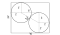
\includegraphics[width=\textwidth]{DiagramaRadioMaximo.pdf}
  \caption{The largest possible radius for $h<w<2h$. From the diagram
    one can see that $t^2+v^2=(2r)^2$, $h=t+2r$ and $w=v+2r$, from which
    one can deduce the value for $r$.}
  \label{radiomaximo}
\end{figure}
We shall look at these regimens on the integration space. The first one is solved
on the main text, but we shall repeat it here with other coordinate system as to
make some points. In figure \ref{diaglimites} we present the three regimens as
the shaded area where we perform the integration. 
  
\begin{figure}[h]
        \centering
        \begin{subfigure}[b]{0.32\textwidth}
          \centering
          \includegraphics[width=\textwidth]{DiagramaIntegraCaso1.pdf}
          \caption{$a,b>r$}
          \label{smallradious}
        \end{subfigure}%
        ~ %add desired spacing between images, e. g. ~, \quad, \qquad etc.
        % (or a blank line to force the subfigure onto a new line)
        \begin{subfigure}[b]{0.32\textwidth}
          \centering
          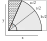
\includegraphics[width=\textwidth]{DiagramaIntegraCaso2.pdf}
          \caption{$b<r$}
          \label{mediumradius}
        \end{subfigure}%
        ~ %add desired spacing between images, e. g. ~, \quad, \qquad etc.
          %(or a blank line to force the subfigure onto a new line)
        \begin{subfigure}[b]{0.32\textwidth}
          \centering
          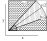
\includegraphics[width=\textwidth]{DiagramaIntegraCaso3.pdf}
          \caption{$a,b<r$}
          \label{bigradious}
        \end{subfigure}%
        \caption{The three posible cases. The shaded area is where the integral
          must be evaluated. In the first case all hopping is possible, the middle case
          only allows for vertical hopping and the last case excludes hopping but there
        is still posibility for the disks to fit inside the table.}
\label{CasosIntegra}
\end{figure}
In the first case (fig. \label{smallradius})  we may use polar coordinates in the
integral on eq. \ref{VolumenGeneral}. As such the indicatrix function becomes
the limits of integration:

\begin{equation}
\begin{split}
V/16 &=\iint \rd x \rd y (2ab-\sqrt{2}(ay+bx)+x y)
\indicator{(x)^2+(y)^2<2r^2 }\\
&=\iint \rd \rho \rd \theta \rho (2ab
-\sqrt{2}(a\rho\sin\theta+b\rho\cos\theta)
+\rho^2 \cos\theta\sin\theta)
\indicator{\rho^2<2r^2 }\\
&=\iint\limits_{0,0}^{\pi/2,r\sqrt{2}} \rd \rho \rd \theta \rho (2ab
-\sqrt{2}(a\rho\sin\theta+b\rho\cos\theta)
+\rho^2 \cos\theta\sin\theta).
\end{split}
\end{equation}

We shall give the definite value for the $\rho$ (radial integration variable),
while leaving the $\theta$ indefinite. This gives us expressions that we can use afterwards:
\begin{equation}\label{volftheta}
\begin{split}
V/16 &=\int\limits_0^{\pi/2}  \rd \theta  
(4abr^2 - r^3 4/3 (a\sin\theta+b*\cos\theta)+r^4 (\cos\theta\sin\theta))\\
&=2abr^2\theta
+\frac{r^34}{3}(a\cos\theta-b\sin\theta)
-\frac{r^4}{4}\cos (2\theta) \bigg\vert_0^{\pi/2} \\
& =abr^2 \pi 
-\frac{4r^3}{3}(a+b)
+\frac{r^4}{2}.
\end{split}
\end{equation}



\section{Acknowledgements}


This work was financed by CONACYT-PAPIIT project number CB-101997.





\bibliography{../../notasmixtas/TwoDiskBiblio}



\end{document}
